\documentclass[16pt, a0paper, landscape,fleqn]{tikzposter}
\usepackage[utf8]{inputenc}
\usepackage{gentium}
\usepackage{amsmath,amsthm, amssymb, latexsym}
\usepackage[american]{babel}
\usepackage{csquotes}
\usepackage[style=apa]{biblatex}
\DeclareLanguageMapping{american}{american-apa}
\addbibresource[location=remote]{https://docs.google.com/uc?id=0B9aB0fj0poVqMzVyYzBGaEdDZG8&export=download}

\title{Absence Makes the Ideal Points Sharper: Full-data IRT Models for Legislatures}
\author{Robert Kubinec}
\date{\today}
\institute{Woodrow Wilson Department of Politics}
\setlength{\mathindent}{1cm}
\usepackage{blindtext}
\usepackage{comment}

\usetheme{Desert}

\begin{document}
	
	\maketitle
	
	\begin{columns}
		\column{0.35}
		\block{Existing IRT 2-PL for Rollcall Data}{
			
			Existing ideal point models based on IRT \parencite{jackman2004} use the following likelihood:
			
			\begin{equation*}
				L(\beta,\alpha,X|Y) = \prod_{n}^{i=1} \prod_{m}^{j=1} \zeta(x_{i}'\beta_j - \alpha_j)^{y_{ij}} \times
				(1 - \zeta(x_{i}'\beta_j - \alpha_j))^{(1-{y_{ij}})}
			\end{equation*}
			
			Where $\beta_j$ represent bill discrimination parameters, $\alpha_j$ represent bill intercepts, $x_i$ are the legislator ideal points and $\zeta$ is a link function (generally logit or probit).
			
			\begin{itemize}
				\item Model assumes that legislators are present at all votes.
				\item Model assumes that all votes are binary (yes or no).
			\end{itemize}
			
			}
				\block{Missing Data?}{
					
			This basic IRT model has been criticized for failing to meet core assumptions about how legislators vote.
			
			\begin{itemize}
				\item Imputation of a missing latent variable is difficult conceptually and practically. In particular, all the assumptions of imputation, such as conditionally missing at random (CMAR), should be met \parencite{rubin2002}. 
				\item I argue that all legislator actions can be interpreted as strategic behavior and can be included without imputation through an appropriate likelihood.
			\end{itemize}
					
				}
				
				\block{Absence-Inflated Ordinal IRT}{
					
					I propose a likelihood that implements a distinct outcome for the $K=3$ possible categories of votes (no, abstain, yes) and the $R \in \{0,1\}$ binary decision to be absent or present. Adopting notation from \textcite{stan2016}, I use an ordered logistic likelihood for vote choice when a legislator is present ($r=1$) such that each outcome is separated by $c \in \mathbb{R}^{K-1}$ cutpoints:
					
					\[
						L(\beta,\alpha,X|Y_{k}) = \prod_{n}^{i=1} \prod_{m}^{j=1}
						\begin{cases} 
						1 -  \zeta(x_{i}'\beta_j - \alpha_j - c_1) & \text{if } K = 0 \\
						\zeta(x_{i}'\beta_j - \alpha_j - c_{k-1}) - \zeta(x_{i}'\beta_j - \alpha_j - c_{k})       & \text{if } 0 < k < K, \text{ and} \\
						\zeta(x_{i}'\beta_j - \alpha_j - c_{k-1}) - 0 & \text{if } k=K
						\end{cases}
					\]
					
					
					This ordinal model is deflated by the probability that a legislator is present  to model the combined $Y_{(k,r)}$ likelihood. The probability of $r=0$ absence is a separate IRT model of common ideal points $x_i$,  and separate bill discrimination/intercepts $\gamma_j$ and $\omega_j$.
					
					 \[
					 L(\beta,\alpha,X,Q,\gamma,\omega|Y_{kr}) = 
					 \prod_{n}^{i=1} \prod_{m}^{j=1}
					 \begin{cases}
					 \zeta({x_{i}'\gamma_j - \omega_j}) & \text{if } r=0, \text{ and} \\
					 (1-\zeta({x_{i}'\gamma_j - \omega_j}))L(\beta,\alpha,X|Y_{k1}) & \text{if } r=1
					 \end{cases}
					 \]
					
					}
		
		\column{0.4}
		\block{Case Study: 114th Senate}{
			In the most recent Senate, modeling absences as an explicit category still largely aligns with the NOMINATE and \texttt{ideal} models that are popularly used for ideal point estimation. This is because of low absence rates (and virtually no absentions) among U.S. Senators.
			\centering
				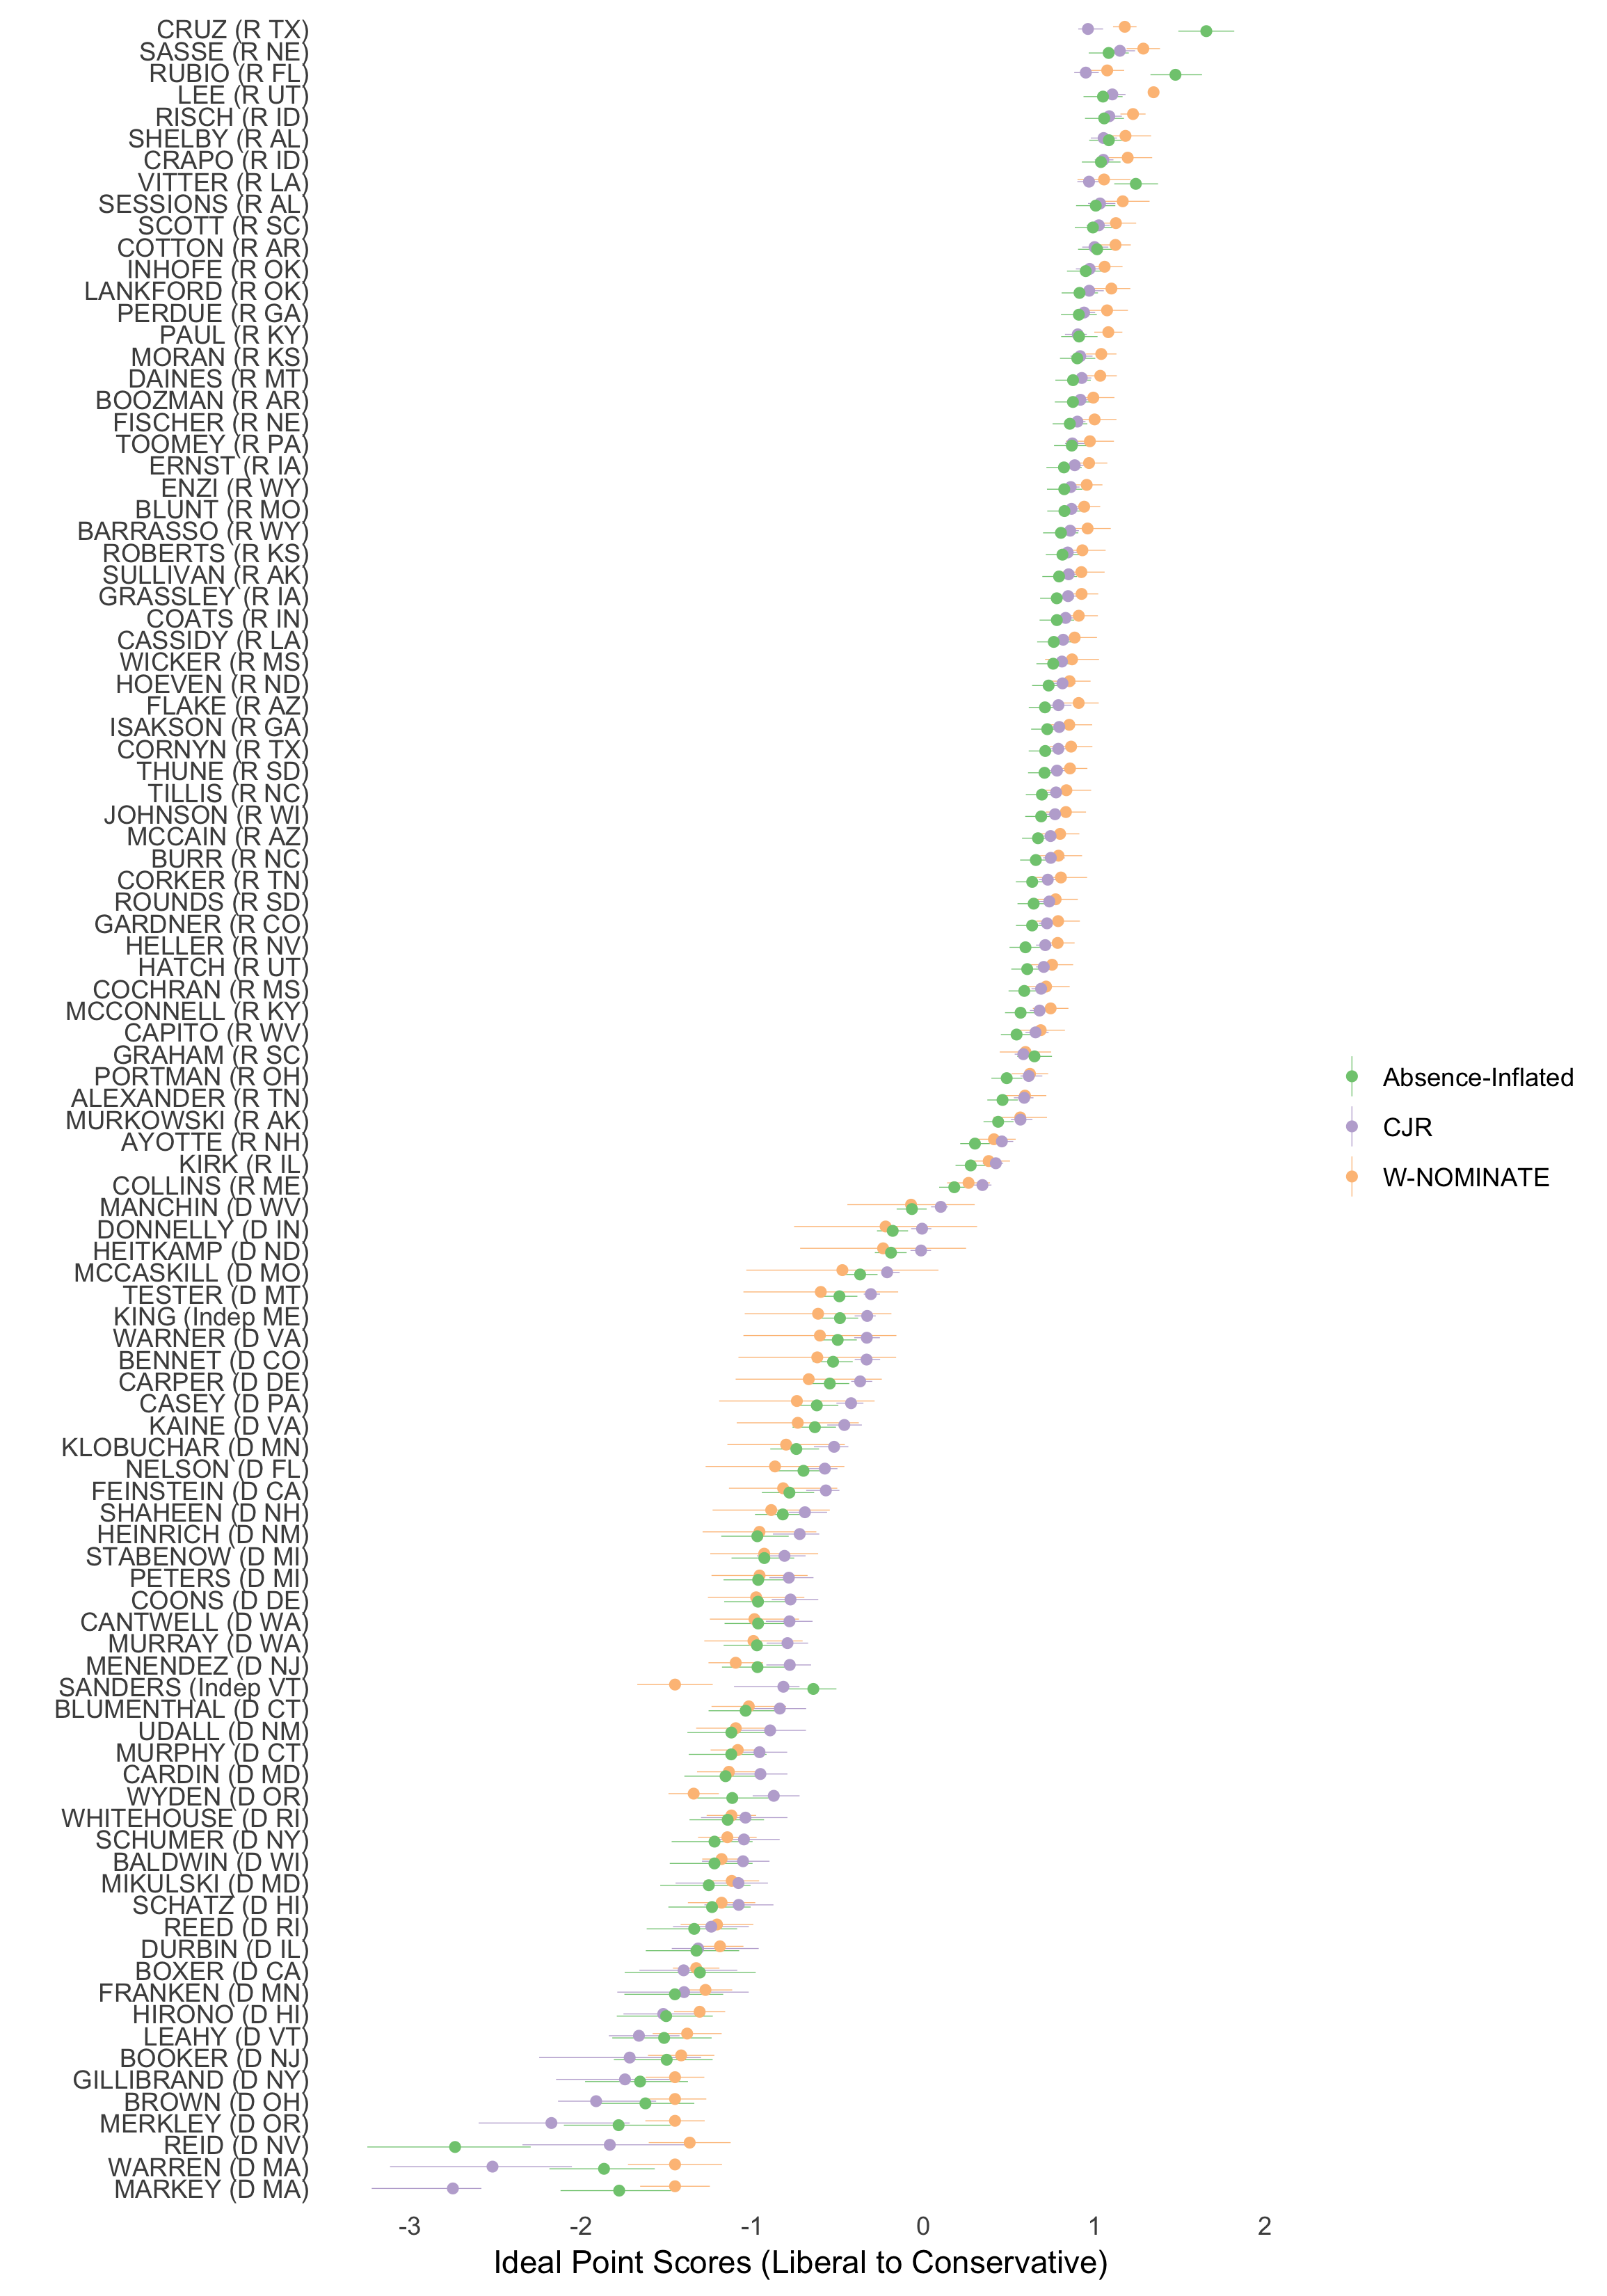
\includegraphics[height=23in]{all_perf}
		
			
			}
		


		


		
		\column{0.25}
		
		\block{}{
	However, ideal points do tend to differ for Senators who were on the campaign trail and had to make strategic decisions about which bills to show up for. Ted Cruz and Marco Rubio all appear far more conservative once their absences are taken into account, while Bernie Sanders is somewhat more moderate. On the other hand, Harry Reid is far more liberal once his absences are taken into account.
	
	
	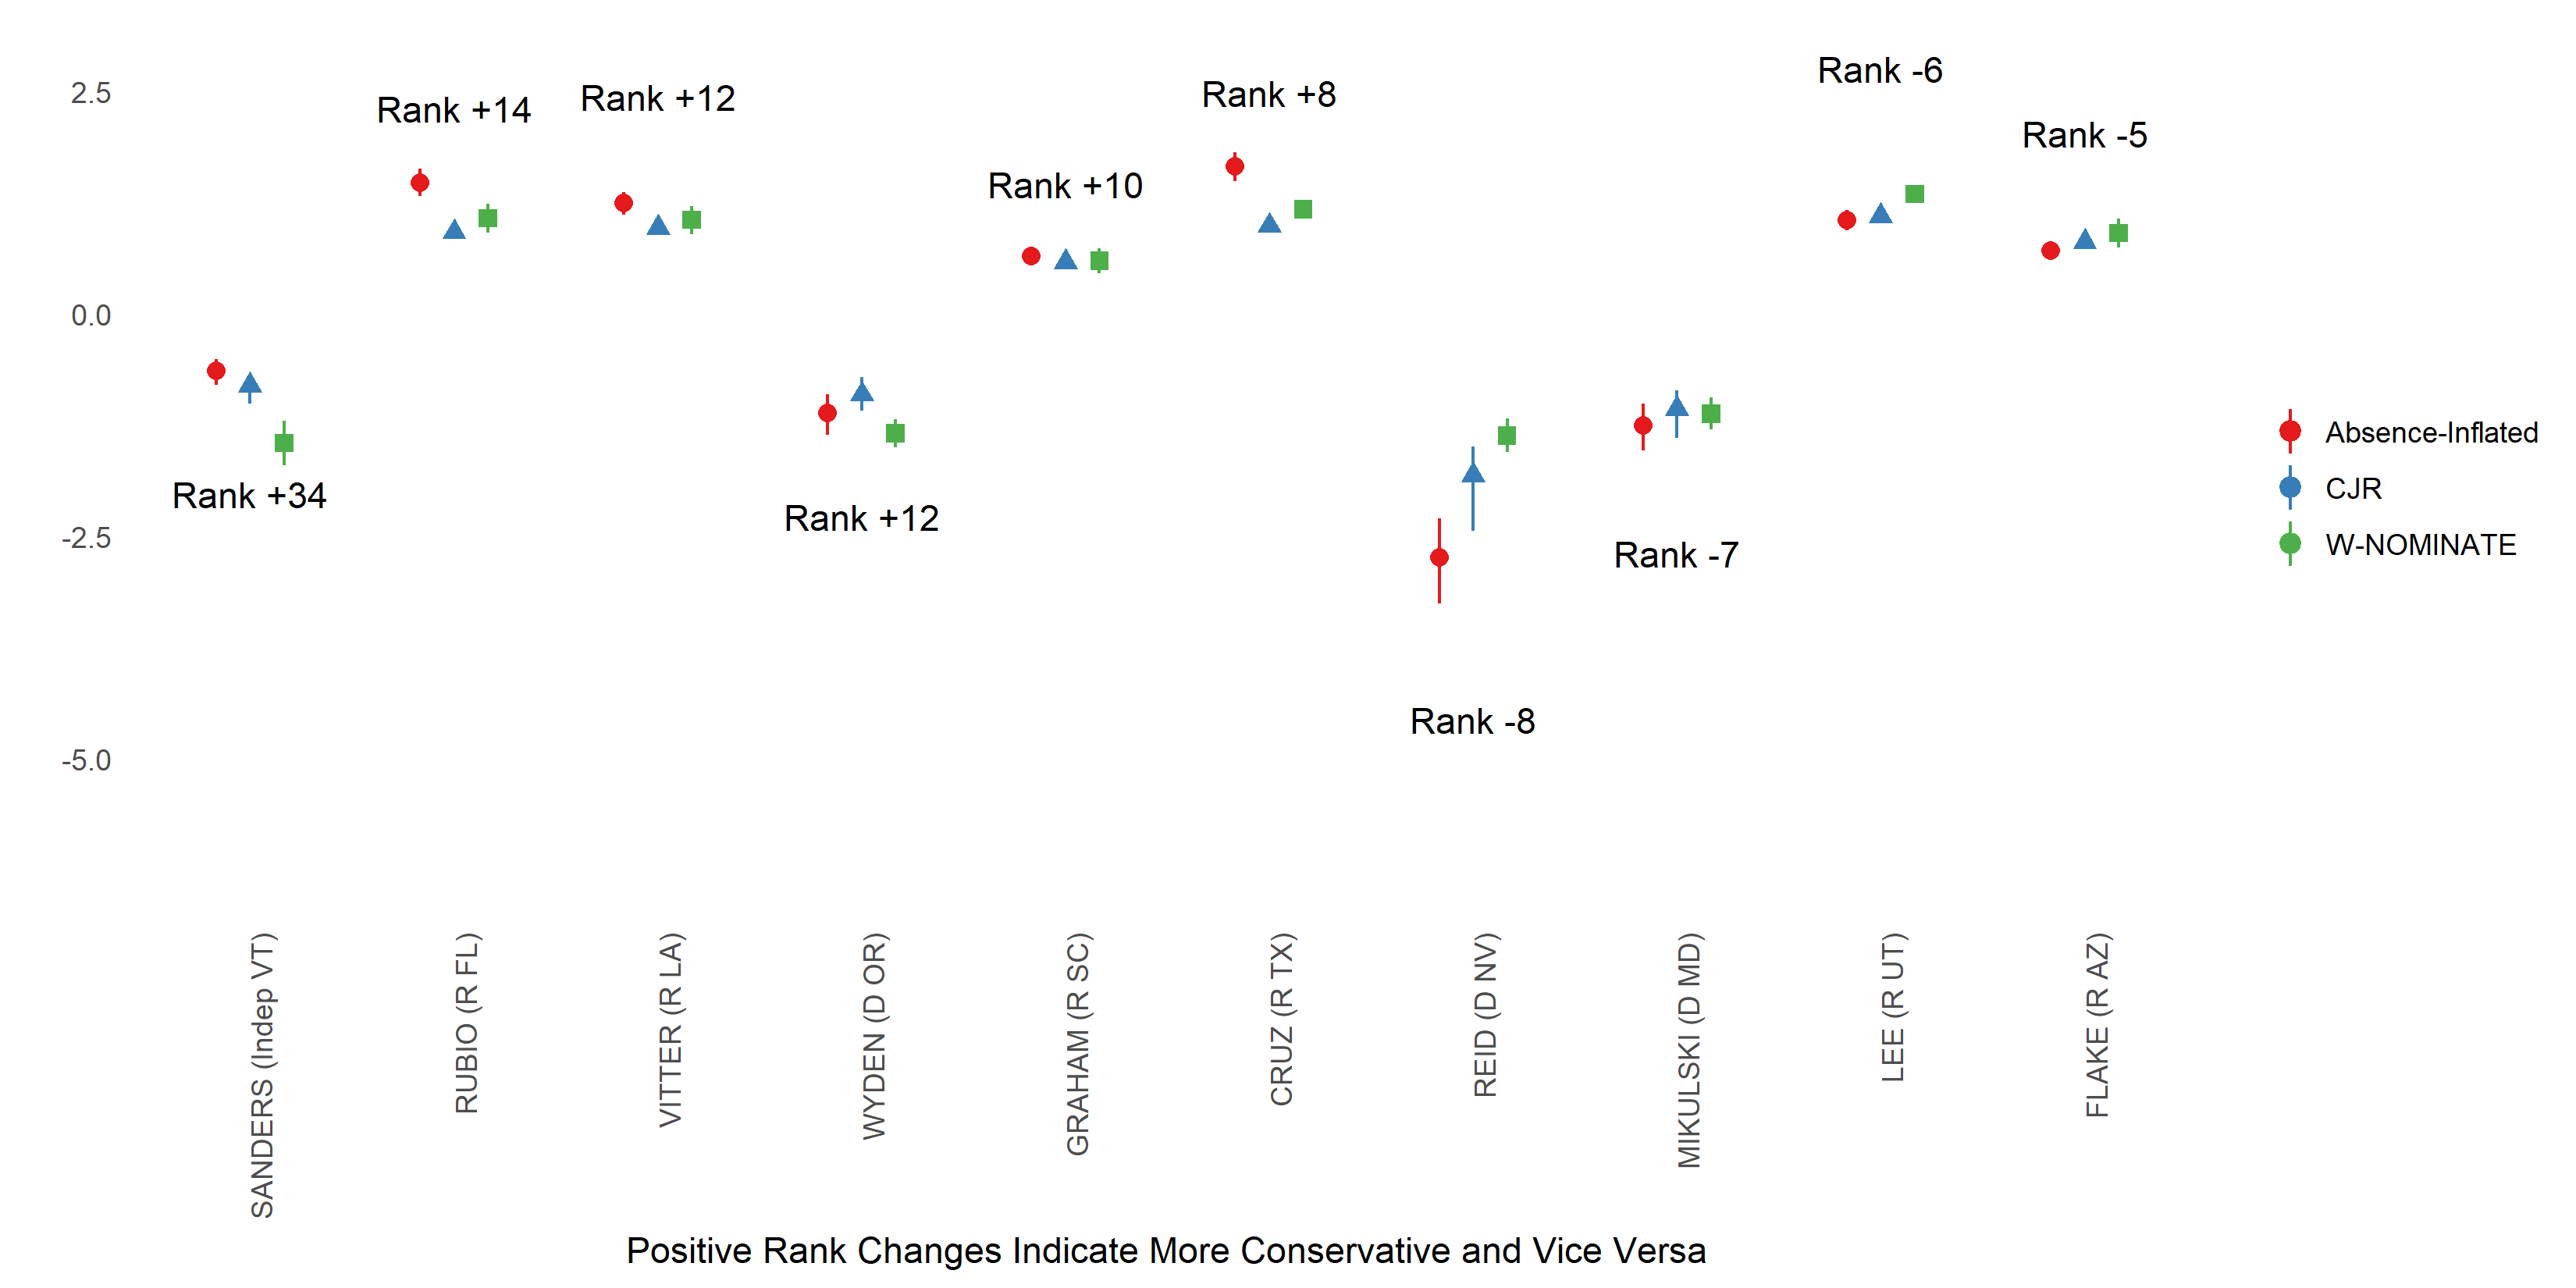
\includegraphics[width=\linewidth]{big_diff}
	
	
}
		
		\block{Case Study: Tunisian Parliament}{
			
			Parliaments with coalition governments can have much higher absentee rates and abstention rates. The data below from Tunisia's legislative assembly, which is considered a transitional democracy, show significantly divering estimates from the standard models.
			\centering
			
			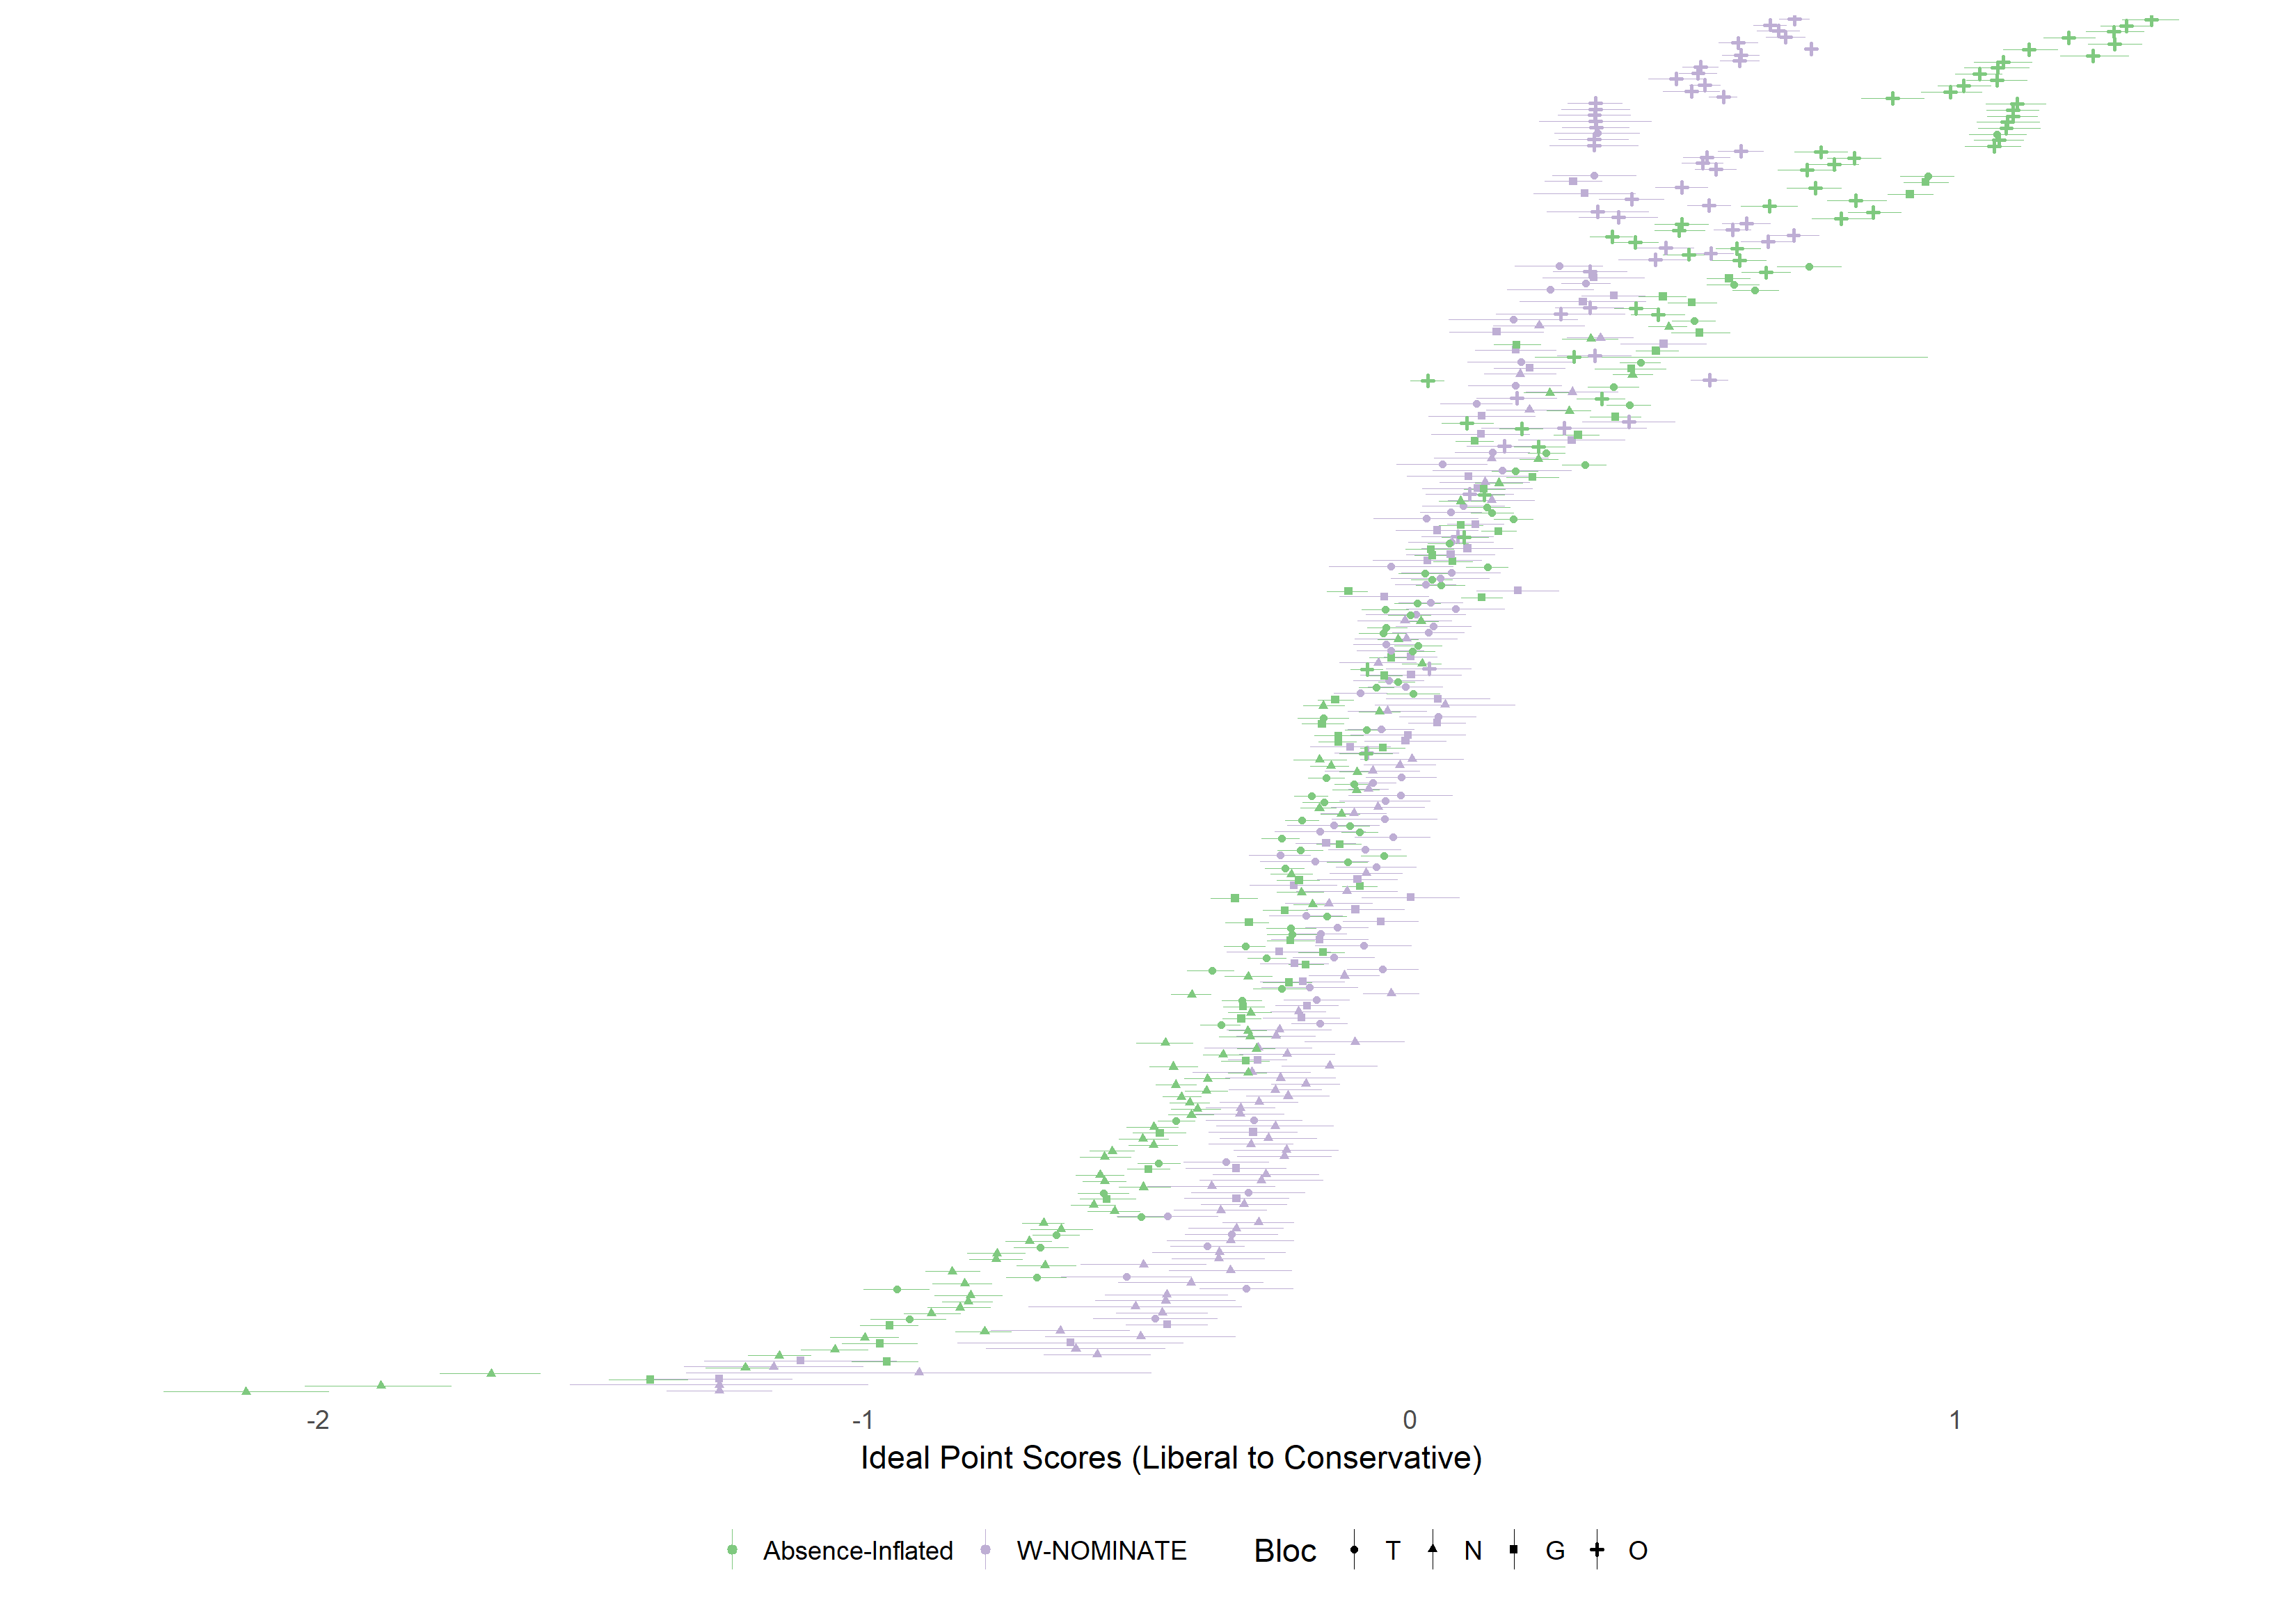
\includegraphics[width=\linewidth]{tunisia_ARP_compare}
			
			}
		
						\block{R Package \texttt{idealstan}}{
			This model and associated plots, along with other IRT ideal point models, are available via the Github-based R package \texttt{idealstan} (www.github.com/saudiwin/idealstan). This package interfaces with the Stan MCMC library for full and approximate Bayesian inference.}
			
			

		

	\end{columns}
	


	
\end{document}